\chapter{Overview}
The CP-even fraction $F_+^{4\pi}$ of \4Pi can be determined through the evaluation of
\begin{equation}
M^{\KsPiPi}_i = h_{\KsPiPi} (T^{\KsPiPi}_i + T^{\KsPiPi}_{-i} - 2 \, c_i  \sqrt{T^{\KsPiPi}_i T^{\KsPiPi}_{-i}} \ (2 F_+^{4\pi} -1))
\end{equation}
and
\begin{equation}
M^{\KlPiPi}_i =  h_{\KlPiPi} (T^{\KlPiPi}_i + T^{\KlPiPi}_{-i} + 2 \, c'_i  \sqrt{T^{\KlPiPi}_i T^{\KlPiPi}_{-i}} \ (2 F_+^{4\pi} -1))
\end{equation}
where the $M_i$ denote the number of events in bin $i$ of the \KsPiPi / \KlPiPi Dalitz-Plot tagged against \4Pi , the $T_i$ the relative amount of events in bin $i$ of flavour-tagged \KsPiPi / \KlPiPi Dalitz-Plot and the $h$ are normalisation factors.\\
By summing over the bins $i$ and $-i$ these expressions become
\begin{equation}
MM^{\KsPiPi}_i = M^{\KsPiPi}_i + M^{\KsPiPi}_{i} =2\cdot h_{\KsPiPi} (T^{\KsPiPi}_i + T^{\KsPiPi}_{-i} - 2 \, c_i  \sqrt{T^{\KsPiPi}_i T^{\KsPiPi}_{-i}} \ (2 F_+^{4\pi} -1))
\end{equation}
and
\begin{equation}
MM^{\KlPiPi}_i = M^{\KlPiPi}_i + M^{\KlPiPi}_{-i} = 2\cdot h_{\KlPiPi} (T^{\KlPiPi}_i + T^{\KlPiPi}_{-i} + 2 \, c'_i  \sqrt{T^{\KlPiPi}_i T^{\KlPiPi}_{-i}} \ (2 F_+^{4\pi} -1))
\end{equation}
The following report summarised how the values for $MM^{\KsPiPi}_i$ and $MM^{\KlPiPi}_i$ are determined.\\


\chapter{Binned \KsPiPi vs \4Pi yields}

\section{Overview}
The values for $MM_i$ are obtained using:
\begin{equation}
MM_i = (N_i^{meas} - B_i^{peak} - B_i^{flat})/ \epsilon_i
\end{equation}
$MM_i$ : absolute number of \4Pi vs \KsPiPi events in bin i. This is the quantity that enters the fit for $F_+$.\\
$N_i^{meas}$ : total number of reconstructed and selected events in bin i. \\
$B_i^{peak}$ : number of reconstructed and selected peaking bkg. events in bin i. The only peaking bkg. expected is \KsPiPi vs \KsPiPi. \\
$B_i^{flat}$ : number of reconstructed and selected flat bkg. events in bin i.\\
$\epsilon_i$ : reconstruction and selection efficiency for \4Pi vs \KsPiPi events in bin i. \\



\section{Raw number of selected \4Pi vs \KsPiPi events }
The selection of \4Pi vs \KsPiPi was done as outlined in Chris' report. The resulting numbers are listed below.\\
\begin{table}[!h]
	\begin{center}
	\begin{tabular}{c| l}
		bin i & $N^{meas}_i\ \pm \sqrt{N^{meas}_i}$  \\
		\hline 
		\hline
1 & 38 $\pm$ 6.16 \\ 
2 & 22 $\pm$ 4.69 \\ 
3 & 21 $\pm$ 4.58 \\ 
4 & 12 $\pm$ 3.46 \\ 
5 & 59 $\pm$ 7.68 \\ 
6 & 24 $\pm$ 4.90  \\ 
7 & 30 $\pm$ 5.48 \\ 
8 & 42 $\pm$ 6.48 \\ 
\end{tabular}
\end{center}
\caption{\textit{Number $N^{meas}_i$ of reconstructed \4Pi vs \KsPiPi events summed over bin i and -i. The errors are taken as $\sqrt{N^{meas}_i}$.}}
\end{table}


\section{Determination of number of peaking background events}
It is assumed that the only peaking bkg to \KsPiPi vs \4Pi is \KsPiPi vs \KsPiPi .\\
The number of peaking bkg events in bin $i$ $B_i^{peak}$ is determined from
\begin{equation}
B_i^{peak} = B_{tot}^{peak} \cdot a_i^{peak}
\end{equation}
where $B_{tot}^{peak}$ denotes the total number of \KsPiPi vs \KsPiPi events in the selected data sample and $a_i^{peak}$ the percentage of \KsPiPi vs \KsPiPi events in bin i.\\

\subsection{Total number of peaking background events in selected data sample}
The total number of peaking bkg events in the selected sample is determined using the generic MC. The same reconstruction and selection as to the data is applied to the generic MC. This results in 60 and 243 selected \KsPiPi vs \KsPiPi events in the lumix10 and lumix20 sample respectively.
\begin{equation}
B_{tot}^{peak}  = 18.45 
\end{equation}

\subsection{Peaking background events per bin}
\label{sec:peak}
Since the generic MC has been generated without taking into account the quantum correlations and no model-dependence should be introduced to the analysis, the relative amount of peaking bkg events per bin has to be determined with data.\\
Therefore the CLEO data is reconstructed and selected in the same way as for the signal decay, apart from a 'reversed \KS veto'. This means that instead of rejecting events where two of the pions from the \4Pi have a \KS flight significance >0, events with a \KS flight significance >2 are selected to ensure a reasonably clean \KsPiPi vs \KsPiPi sample.\\
Unfortunately 'reversed \KS veto' introduced a bias in the distribution of expected \KsPiPi vs \KsPiPi events over the bins. Figure \ref{fig:selbias} shows the distribution of \KsPiPi vs \KsPiPi events over the bins for the selection with the \KS-Veto and the 'reversed \KS veto' on \KsPiPi vs \KsPiPi signal MC.\\
\newpage
\begin{figure}[!h]
	\vspace*{-0.cm}
	\begin{center}
		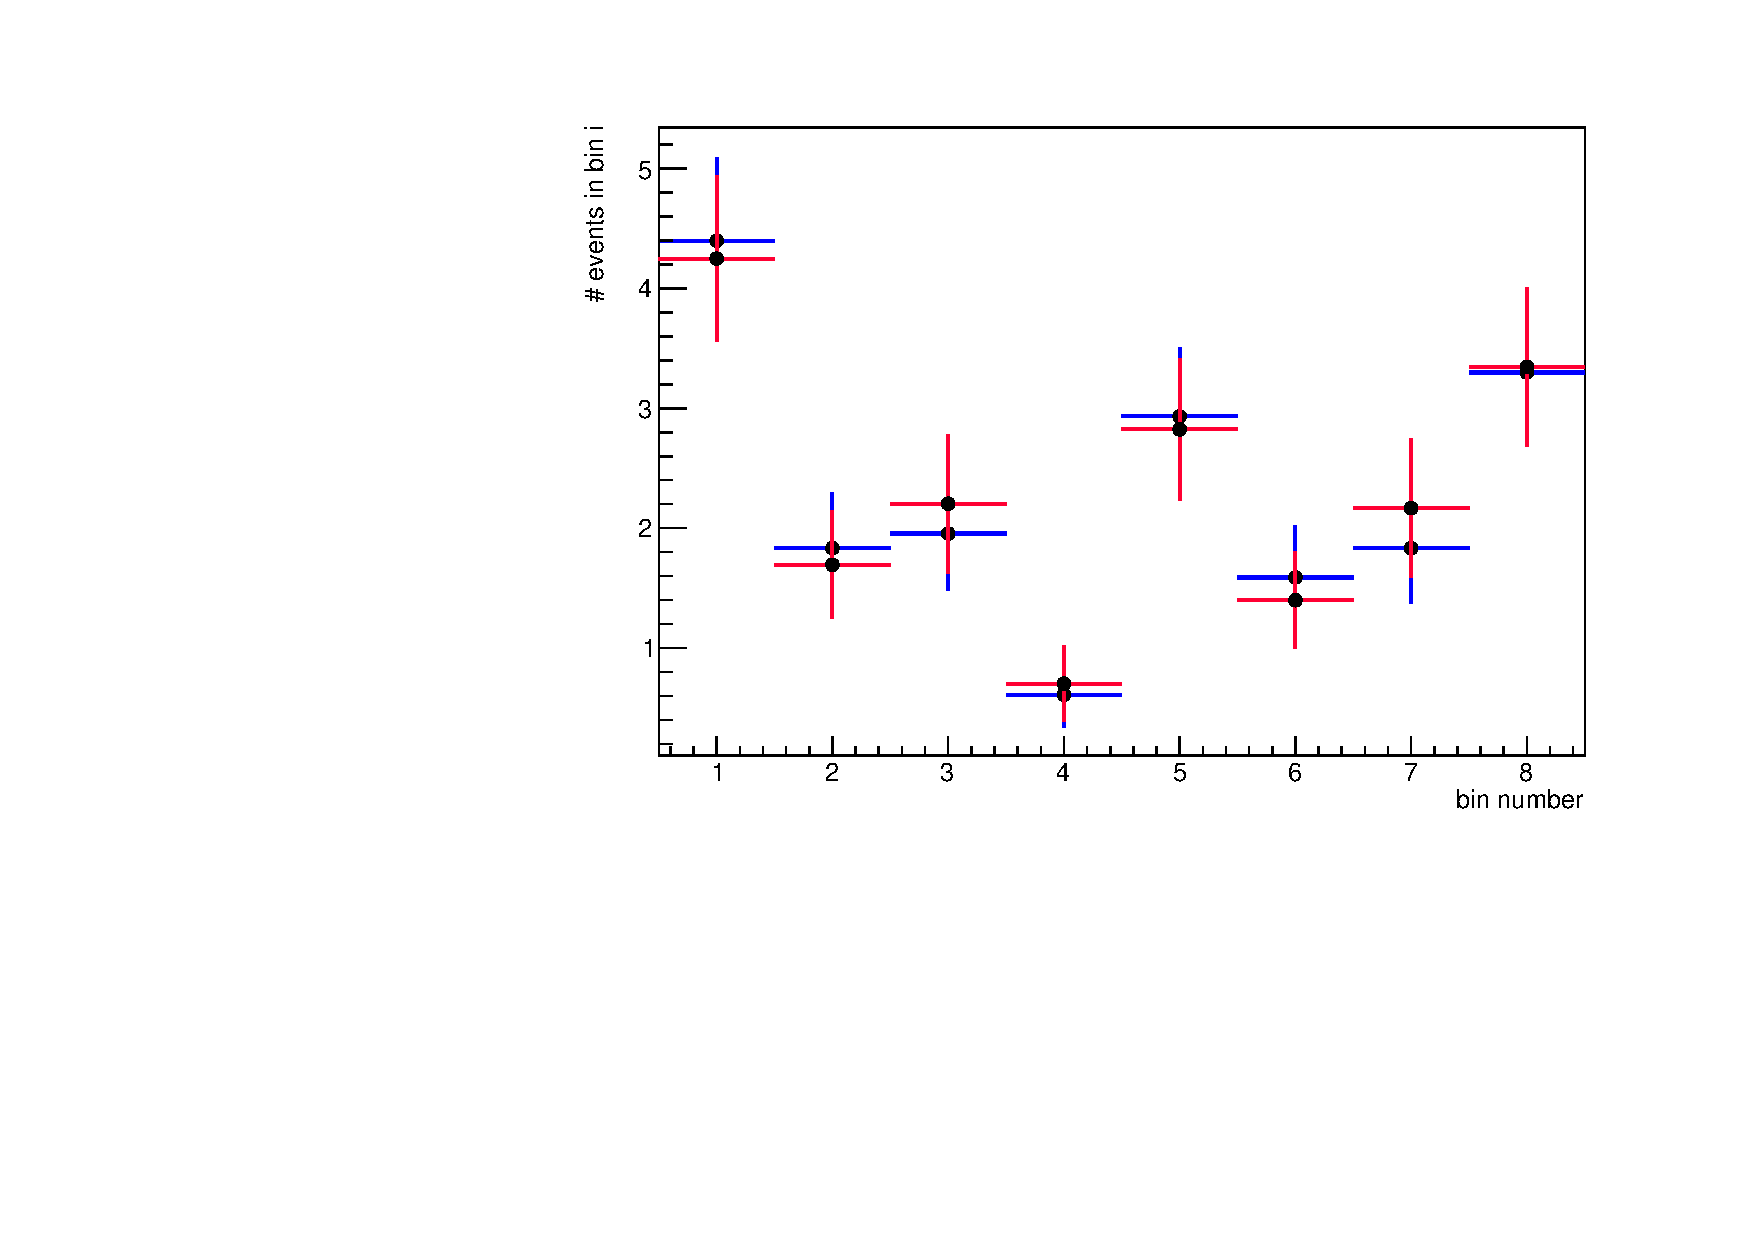
\includegraphics[width=1.\textwidth]{KsPiPi_selbias.pdf}
		\vspace*{-1.5cm}
	\end{center}
	\caption{\textit{Distribution of \KsPiPi vs \KsPiPi events over the bins determined by using \KsPiPi vs \KsPiPi MC. Blue: reversed \KS veto cut of FS>2, red: \KS veto cut of FS<0 as is used in the data sample.}}
	\label{fig:selbias}
\end{figure}
To compensate for this bias the values for the percentage of \KsPiPi vs \KsPiPi per bins obtained from the data are being weighted with the ratio of reversed \KS veto over the \KS veto efficiencies determined from the \KsPiPi vs \KsPiPi signal MC sample. This yields the total amount of \KsPiPi vs \KsPiPi contamination in the data sample listed below.
\begin{table}[!h]
	\begin{center}
		\begin{tabular}{c| l}
			bin i & $B^{peak}_i$  \\
			\hline 
			\hline
1 & 4.21854 $\pm$ 2 $\oplus$ 0.637882 \\ 
2 & 1.68165 $\pm$ 1.5 $\oplus$ 0.434214 \\ 
3 & 2.18858 $\pm$ 1.5 $\oplus$ 0.559566 \\ 
4 & 0.697849 $\pm$ 0.5 $\oplus$ 0.314724 \\ 
5 & 2.80305 $\pm$ 1.5 $\oplus$ 0.562877 \\ 
6 & 1.38776 $\pm$ 1.5 $\oplus$ 0.391982 \\ 
7 & 2.15081 $\pm$ 1.5 $\oplus$ 0.559324 \\ 
8 & 3.32175 $\pm$ 1.5 $\oplus$ 0.624964 \\
	\end{tabular}
	\end{center}
	\caption{\textit{Number of peaking background events per bin in the data sample. The first error is the Poisson error on the yields, the second error comes from the systematic uncertainty on the distribution over the bins.}}
	\vspace*{1cm}
\end{table}


\subsubsection{Cleanness of \KsPiPi vs \KsPiPi sample}
\label{sec:clean}
The gen MC suggest that the 'reversed \KS veto' yields a sample of 96\% \KsPiPi vs \KsPiPi events. The rest is distributed as follows:
\begin{itemize}
\item 2.8\% \4Pi vs \KsPiPi 
\item 0.2\% flat				
\item 1.0\% \KsPiPi vs \KsKs (with the \KsKs on the \KsPiPi side)
\end{itemize}
This will be accounted for in the systematic uncertainties in Section \ref{s:peakb}.\\

\section{Determination of number of flat background events}
\label{sec:flat}
The number of flat bkg events is determined using the usual sidebands (denoted A, B, C and D). The number of events in the sidebands is extrapolated to give the amount of flat bkg in the signal region using the equation
\begin{equation}
B_{tot}^{flat} = \frac{a_S}{a_D}N_D +  \sum_{j = A,B,C} \frac{a_S}{a_j} (N_j - \frac{a_j}{a_D}N_D)
\end{equation}
where $N_j$ is the number of events in sideband j, $a_j$ is the area of sideband j and $a_S$ is the area of the signal region. The results are listed below (no errors are assumed on the values of $a_j$).  
\begin{table}[!h]
	\begin{center}
		\begin{tabular}{c| c}
     $N_A$ & 1  \\
     $N_B$ & 0 \\
     $N_C$ & 20  \\
     $N_D$ & 2 \\
     \hline
     $B_{tot}^{flat}$  & 11.64  \\
    	\end{tabular}
	    \vspace*{-0.5cm}
    \end{center}
    \caption{\textit{Number of flat bkg in the sideband and extrapolated to the signal region.}}
\end{table}
  
To get the number of flat bkg events in bin i, the relative area of bin i is determined using the \texttt{dkpp\_babar.root} histogram. Assuming no error on the relative area of bin i the number of flat bkg events are:
\clearpage
\begin{table}[!h]
	\begin{center}
		\begin{tabular}{c| c}
			bins & number of flat bkg events \\
			\hline
1 & 3.85 $\pm$ 2 \\ 
2 & 1.33 $\pm$ 1 \\ 
3 & 0.74 $\pm$ 1 \\ 
4 & 0.69 $\pm$ 0.5 \\ 
5 & 1.55 $\pm$ 1.5 \\ 
6 & 0.94 $\pm$ 1 \\ 
7 & 0.98 $\pm$ 1 \\ 
8 & 1.56 $\pm$ 1.5 \\ 
	\end{tabular}
 \vspace*{-0.5cm}
\end{center}
\caption{\textit{Number of flat bkg events per bin.}}
\end{table} 

\section{Determination of the signal selection-efficiency}
The signal selection efficiency in each bin is determined using a sample of 266998 \KsPiPi vs \4Pi signal MC events.\\
%The signal selection efficiency in each bin is determined using a combination the efficiency of \KtPi vs \KsPiPi determined in an earlier analysis and \KsPiPi vs \4Pi signal MC. The signal MC is used to calculate the absolute selection efficiency while the efficiencies from \KtPi vs \KsPiPi are used to scale between the bins.\\
\begin{table}[!h]
	\begin{center}
		\begin{tabular}{c| l }
			bin & $\epsilon$  \\
			\hline
1 & 0.1553 $\pm$ 0.0012 \\ 
2 & 0.1529 $\pm$ 0.0021 \\ 
3 & 0.1761 $\pm$ 0.0029 \\ 
4 & 0.1671 $\pm$ 0.0030 \\ 
5 & 0.1583 $\pm$ 0.0019 \\ 
6 & 0.1642 $\pm$ 0.0025 \\ 
7 & 0.1551 $\pm$ 0.0024 \\ 
8 & 0.1607 $\pm$ 0.0020 \\
			\end{tabular}
	\end{center}
	\vspace*{-0.5cm}
	\caption{\textit{Signal efficiency per bin.}}
\end{table}

\clearpage
\section{Bkg substracted, efficiency corrected, rescaled signal yields}
\begin{table}[!h]
	\begin{center}
		\begin{tabular}{c| c }
			bin & $MM_i$  \\
			\hline
1 & 30.7804 $\pm$ 6.97383 $\oplus$ 0.241629 $\oplus$ 0.655893 \\ 
2 & 19.8284 $\pm$ 5.24652 $\oplus$ 0.26636 $\oplus$ 0.453361 \\ 
3 & 16.3846 $\pm$ 4.46561 $\oplus$ 0.273724 $\oplus$ 0.50743 \\ 
4 & 10.1474 $\pm$ 3.37991 $\oplus$ 0.180279 $\oplus$ 0.300871 \\ 
5 & 55.1394 $\pm$ 8.04054 $\oplus$ 0.676977 $\oplus$ 0.567952 \\ 
6 & 21.0775 $\pm$ 5.07712 $\oplus$ 0.325249 $\oplus$ 0.381242 \\ 
7 & 27.6736 $\pm$ 5.93899 $\oplus$ 0.432454 $\oplus$ 0.576076 \\ 
8 & 36.8818 $\pm$ 6.77579 $\oplus$ 0.448323 $\oplus$ 0.620996 \\ 
	\end{tabular}
\end{center}
\vspace*{-0.5cm}
\caption{\textit{$M_i$ + $M_{-i}$ The first error is the Poisson error on the raw data yields and the bkg yields, the second error comes from the limited data and MC samples used to determine the distribution of peaking bkg events and the third from the signal efficiency.}}
\label{tab:MMKs}
\end{table} 

\section{Summary}
\begin{table}[!h]
	\begin{center}
		\begin{tabular}{c| c | c | c|c}
		bin & raw yields & $B^{peak}_i$ & $B^{flat}_i$ &  signal  \\
		\hline 
		\hline
1 & 38 & 4.219 & 3.846 & 30.78 \\ 
2 & 22 & 1.682 & 1.327 & 19.83 \\ 
3 & 21 & 2.189 & 0.7433 & 16.38 \\ 
4 & 12 & 0.6978 & 0.6875 & 10.15 \\ 
5 & 59 & 2.803 & 1.55 & 55.14 \\ 
6 & 24 & 1.388 & 0.941 & 21.08 \\ 
7 & 30 & 2.151 & 0.9804 & 27.67 \\ 
8 & 42 & 3.322 & 1.561 & 36.88 \\ 
		\end{tabular}
	\end{center}
	\caption{\textit{Summary of contributions to the raw yields per bin.}}
\end{table}


